\usetikzlibrary{shapes.geometric}
\begin{figure}[H]
\centering
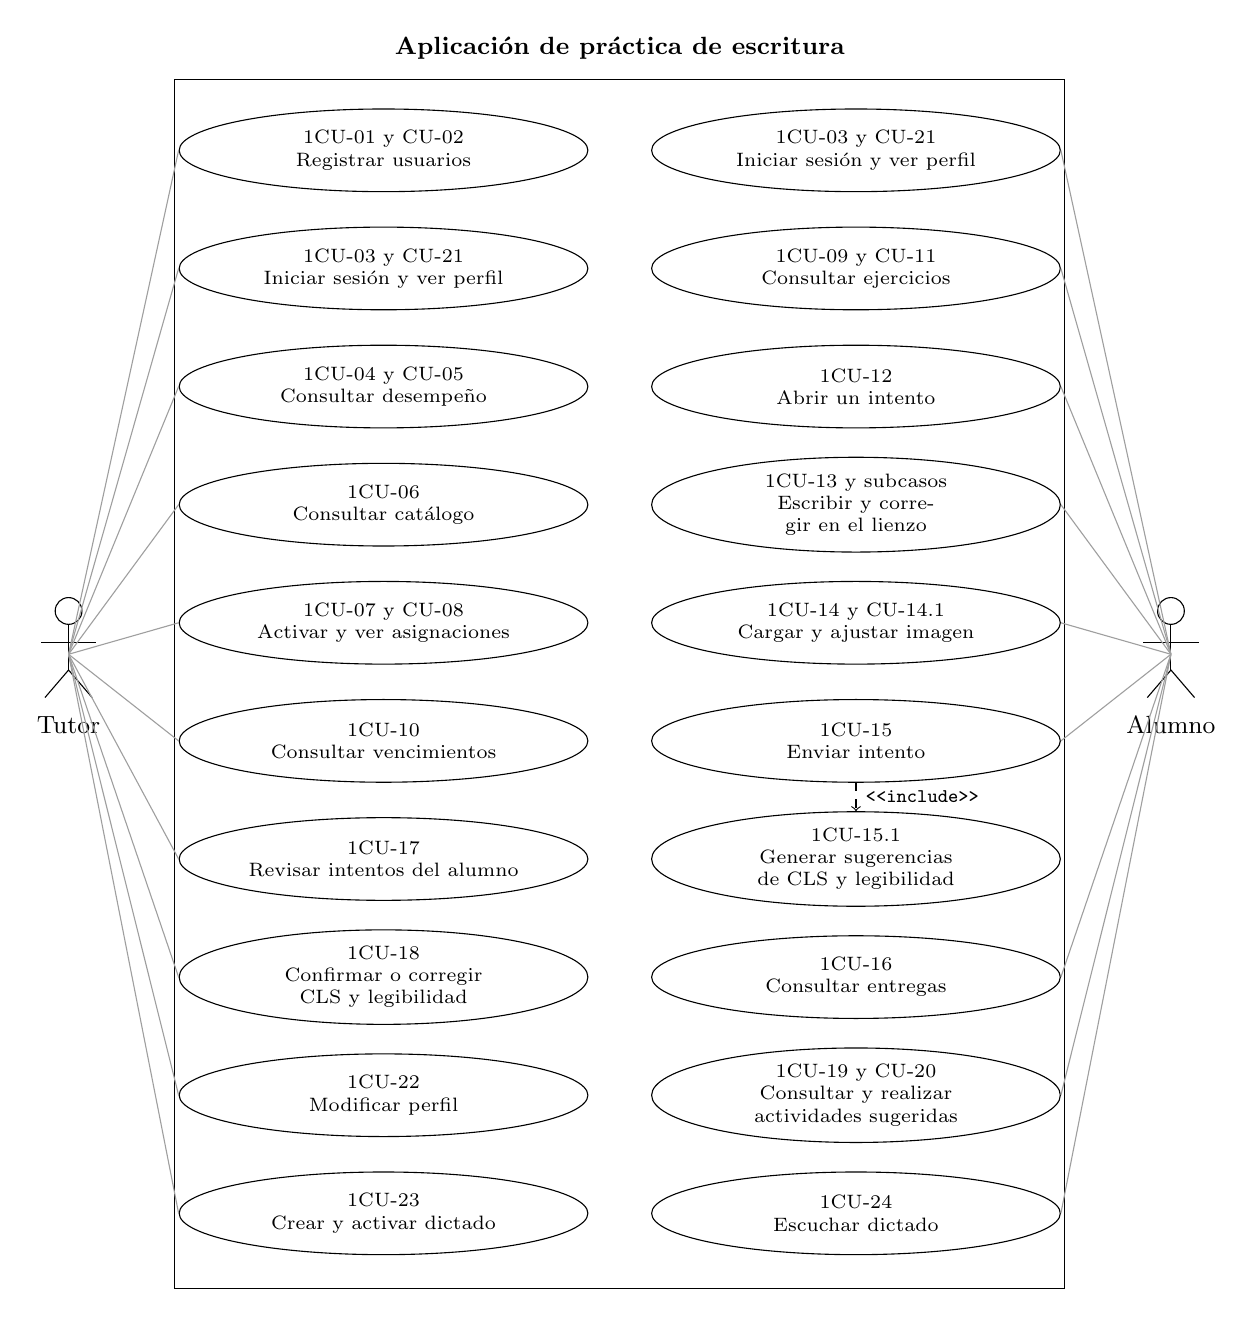
\begin{tikzpicture}[
    caso/.style={draw,ellipse,align=center,text width=3.6cm,
        font=\scriptsize\setstretch{1},inner sep=1pt,minimum height=1.05cm},
    enlace/.style={thin,gray!75}
]
\draw (1.35,0.25) rectangle (12.65,-15.1);
\node[font=\small\bfseries] at (7,0.65) {Aplicación de práctica de escritura};

\draw (0,-6.5) circle (0.17);
\draw (0,-6.67) -- (0,-7.25);
\draw (-0.35,-6.9) -- (0.35,-6.9);
\draw (-0.3,-7.6) -- (0,-7.25) -- (0.3,-7.6);
\node[font=\small] at (0,-7.95) {Tutor};
\coordinate (tutor) at (0,-7.05);

\draw (14,-6.5) circle (0.17);
\draw (14,-6.67) -- (14,-7.25);
\draw (13.65,-6.9) -- (14.35,-6.9);
\draw (13.7,-7.6) -- (14,-7.25) -- (14.3,-7.6);
\node[font=\small] at (14,-7.95) {Alumno};
\coordinate (alumno) at (14,-7.05);

\node[caso] (t1) at (4,-0.65) {CU-01 y CU-02\\Registrar usuarios};
\node[caso] (t2) at (4,-2.15) {CU-03 y CU-21\\Iniciar sesión y ver perfil};
\node[caso] (t3) at (4,-3.65) {CU-04 y CU-05\\Consultar desempeño};
\node[caso] (t4) at (4,-5.15) {CU-06\\Consultar catálogo};
\node[caso] (t5) at (4,-6.65) {CU-07 y CU-08\\Activar y ver asignaciones};
\node[caso] (t6) at (4,-8.15) {CU-10\\Consultar vencimientos};
\node[caso] (t7) at (4,-9.65) {CU-17\\Revisar intentos del alumno};
\node[caso] (t8) at (4,-11.15) {CU-18\\Confirmar o corregir\\CLS y legibilidad};
\node[caso] (t9) at (4,-12.65) {CU-22\\Modificar perfil};
\node[caso] (t10) at (4,-14.15) {CU-23\\Crear y activar dictado};

\node[caso] (a1) at (10,-0.65) {CU-03 y CU-21\\Iniciar sesión y ver perfil};
\node[caso] (a2) at (10,-2.15) {CU-09 y CU-11\\Consultar ejercicios};
\node[caso] (a3) at (10,-3.65) {CU-12\\Abrir un intento};
\node[caso] (a4) at (10,-5.15) {CU-13 y subcasos\\Escribir y corregir en el lienzo};
\node[caso] (a5) at (10,-6.65) {CU-14 y CU-14.1\\Cargar y ajustar imagen};
\node[caso] (a6) at (10,-8.15) {CU-15\\Enviar intento};
\node[caso] (analisis) at (10,-9.65) {CU-15.1\\Generar sugerencias\\de CLS y legibilidad};
\node[caso] (a7) at (10,-11.15) {CU-16\\Consultar entregas};
\node[caso] (a8) at (10,-12.65) {CU-19 y CU-20\\Consultar y realizar\\actividades sugeridas};
\node[caso] (a9) at (10,-14.15) {CU-24\\Escuchar dictado};

\foreach \n in {t1,t2,t3,t4,t5,t6,t7,t8,t9,t10}
    \draw[enlace] (tutor) -- (\n.west);
\foreach \n in {a1,a2,a3,a4,a5,a6,a7,a8,a9}
    \draw[enlace] (alumno) -- (\n.east);
\draw[dashed,->] (a6.south) -- node[right,font=\scriptsize]{\texttt{<<include>>}} (analisis.north);
\end{tikzpicture}
\caption{Vista resumida de los casos de uso por actor. Los casos relacionados se agrupan para facilitar la lectura; sus condiciones se detallan en las fichas.}
\label{fig:casos_uso}
\end{figure}
